\chapter[Sprint II]{Study and Implementation of Sprint II: Authentication \& Landing Page}

\minitoc

\section{Introduction}
This chapter presents the study and implementation of Sprint II, which focuses on developing the authentication system and landing page for our application. The sprint encompasses the integration of modern authentication mechanisms using NextAuth.js and database management with Prisma, along with the creation of an intuitive landing page that serves as the entry point for users. This sprint builds upon the foundation established in previous iterations and introduces essential user management capabilities that form the backbone of the application's security architecture.

\section{Sprint Planning}

\subsection{Objectives of Sprint II}
The primary objectives of Sprint II include:
\begin{itemize}
    \item Implement secure user authentication using OAuth providers (Google, GitHub)
    \item Develop session management for cross-device authentication persistence
    \item Create an engaging and responsive landing page
    \item Establish database schema and ORM integration using Prisma
    \item Ensure seamless user sign-in and sign-out functionality
    \item Implement user session persistence across multiple devices
\end{itemize}

\subsection{Backlog of Sprint II}
% Note: Import backlog1.csv and filter for third column value < 2
\begin{table}[H]
\centering
\caption{Sprint II Backlog Items}
\label{tab:sprint2_backlog}
\begin{tabular}{|p{1cm}|p{6cm}|p{2cm}|p{2cm}|p{2cm}|}
\hline
\textbf{ID} & \textbf{User Story} & \textbf{Priority} & \textbf{Effort} & \textbf{Status} \\
\hline
% TODO: Insert filtered CSV data where third column < 2
% Example rows:
1 & As a user, I want to sign in with Google account & 1 & 5 & Completed \\
\hline
2 & As a user, I want to sign in with GitHub account & 1 & 3 & Completed \\
\hline
3 & As a user, I want to stay authenticated across devices & 1 & 8 & Completed \\
\hline
4 & As a user, I want to sign out from my account & 1 & 2 & Completed \\
\hline
5 & As a visitor, I want to explore the landing page & 1 & 5 & Completed \\
\hline
\end{tabular}
\end{table}

\section{Technologies and Tools Used}

\subsection{NextAuth.js}
NextAuth.js is a comprehensive authentication library designed specifically for Next.js applications. It provides a complete authentication solution with support for multiple OAuth providers, database adapters, and session management strategies. The library offers built-in security features including CSRF protection, JWT tokens, and secure cookie handling. NextAuth.js simplifies the implementation of authentication flows while maintaining high security standards and providing flexibility for customization.

\subsection{Prisma}
Prisma is a next-generation Object-Relational Mapping (ORM) tool that provides type-safe database access for Node.js applications. It offers a declarative schema definition language, automatic migration generation, and a powerful query engine. Prisma's integration with TypeScript ensures compile-time type safety and excellent developer experience through auto-completion and IntelliSense. The tool supports multiple database providers and simplifies complex database operations while maintaining optimal performance.

\section{Analyse}

\subsection{Use case diagram for Sprint II}
\begin{figure}[H]
    \centering
    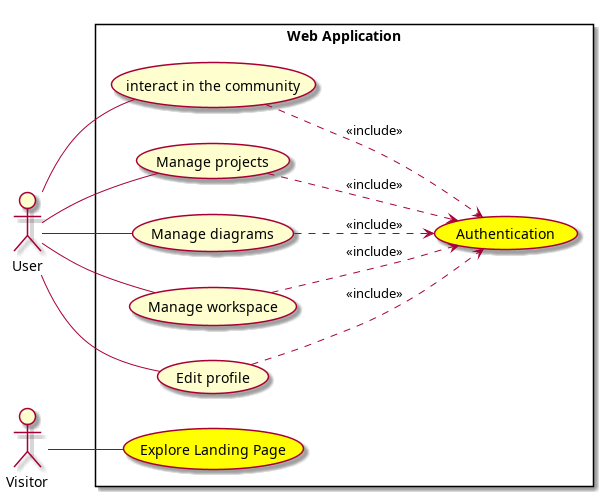
\includegraphics[width=0.8\textwidth]{conception/SprintII/use_case_diagrams/use_case_diagram_of_SprintII.png}
    \caption{Use Case Diagram for Sprint II}
    \label{fig:usecase_sprint2}
\end{figure}

The use case diagram for Sprint II illustrates the main interactions between users and the authentication system, highlighting the key functionalities implemented during this sprint.

\subsection{Refined use case "Authentication"}
\begin{figure}[H]
    \centering
    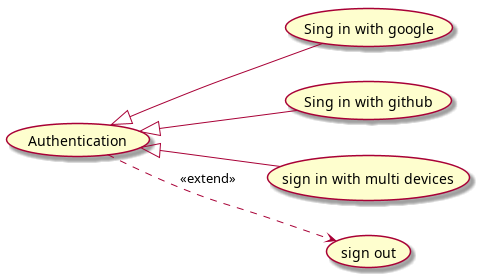
\includegraphics[width=0.8\textwidth]{conception/SprintII/use_case_diagrams/refined_use_case_feature_auth.png}
    \caption{Refined Use Case Diagram for Authentication Feature}
    \label{fig:refined_auth_usecase}
\end{figure}

\subsubsection{Use case}
The authentication use case encompasses all user authentication-related activities including sign-in through OAuth providers, session management, and sign-out functionality.

\subsubsection{Textual description of use case}

\textbf{Use Case: Sign in with Google Account}
\begin{table}[H]
\centering
\caption{Textual Description - Sign in with Google Account}
\label{tab:google_signin_description}
\begin{tabular}{|p{3cm}|p{10cm}|}
\hline
\textbf{Use Case Name} & Sign in with Google Account \\
\hline
\textbf{Primary Actor} & User \\
\hline
\textbf{Goal} & Authenticate user using Google OAuth \\
\hline
\textbf{Preconditions} & User has a valid Google account \\
\hline
\textbf{Main Flow} & 
1. User clicks "Sign in with Google" button \\
& 2. System redirects to Google OAuth page \\
& 3. User enters Google credentials \\
& 4. Google validates credentials \\
& 5. System receives authorization code \\
& 6. System creates user session \\
& 7. User is redirected to dashboard \\
\hline
\textbf{Alternative Flow} & 
A1. Invalid credentials: Display error message \\
& A2. OAuth cancelled: Return to sign-in page \\
\hline
\textbf{Postconditions} & User is authenticated and session is created \\
\hline
\end{tabular}
\end{table}

\textbf{Use Case: Sign in with GitHub Account}
\begin{table}[H]
\centering
\caption{Textual Description - Sign in with GitHub Account}
\label{tab:github_signin_description}
\begin{tabular}{|p{3cm}|p{10cm}|}
\hline
\textbf{Use Case Name} & Sign in with GitHub Account \\
\hline
\textbf{Primary Actor} & User \\
\hline
\textbf{Goal} & Authenticate user using GitHub OAuth \\
\hline
\textbf{Preconditions} & User has a valid GitHub account \\
\hline
\textbf{Main Flow} & 
1. User clicks "Sign in with GitHub" button \\
& 2. System redirects to GitHub OAuth page \\
& 3. User authorizes application access \\
& 4. GitHub returns authorization code \\
& 5. System validates and creates session \\
& 6. User is redirected to dashboard \\
\hline
\textbf{Alternative Flow} & 
A1. Authorization denied: Return to sign-in page \\
& A2. Network error: Display retry option \\
\hline
\textbf{Postconditions} & User is authenticated with GitHub identity \\
\hline
\end{tabular}
\end{table}

\textbf{Use Case: Stay Authenticated Across Multiple Devices}
\begin{table}[H]
\centering
\caption{Textual Description - Cross-Device Authentication}
\label{tab:cross_device_auth_description}
\begin{tabular}{|p{3cm}|p{10cm}|}
\hline
\textbf{Use Case Name} & Stay Authenticated Across Multiple Devices \\
\hline
\textbf{Primary Actor} & Authenticated User \\
\hline
\textbf{Goal} & Maintain authentication state across devices \\
\hline
\textbf{Preconditions} & User is authenticated on one device \\
\hline
\textbf{Main Flow} & 
1. User signs in on Device A \\
& 2. System creates persistent session \\
& 3. User accesses application on Device B \\
& 4. System validates session token \\
& 5. User gains access without re-authentication \\
\hline
\textbf{Alternative Flow} & 
A1. Session expired: Redirect to sign-in \\
& A2. Security breach detected: Force re-authentication \\
\hline
\textbf{Postconditions} & User maintains access across devices \\
\hline
\end{tabular}
\end{table}

\textbf{Use Case: Sign Out}
\begin{table}[H]
\centering
\caption{Textual Description - Sign Out}
\label{tab:signout_description}
\begin{tabular}{|p{3cm}|p{10cm}|}
\hline
\textbf{Use Case Name} & Sign Out From Account \\
\hline
\textbf{Primary Actor} & Authenticated User \\
\hline
\textbf{Goal} & Terminate user session securely \\
\hline
\textbf{Preconditions} & User is currently authenticated \\
\hline
\textbf{Main Flow} & 
1. User clicks sign-out button \\
& 2. System invalidates current session \\
& 3. System clears authentication tokens \\
& 4. User is redirected to landing page \\
\hline
\textbf{Alternative Flow} & 
A1. Network error: Local session cleared \\
\hline
\textbf{Postconditions} & User session is terminated \\
\hline
\end{tabular}
\end{table}

\subsection{Refined use case "Explore Landing Page"}
\subsubsection{Use case}
The landing page exploration use case covers the visitor's interaction with the application's entry point, including navigation, information consumption, and call-to-action engagement.

\subsubsection{Textual description of use case}
\begin{table}[H]
\centering
\caption{Textual Description - Explore Landing Page}
\label{tab:landing_page_description}
\begin{tabular}{|p{3cm}|p{10cm}|}
\hline
\textbf{Use Case Name} & Explore Landing Page \\
\hline
\textbf{Primary Actor} & Visitor \\
\hline
\textbf{Goal} & Learn about the application and its features \\
\hline
\textbf{Preconditions} & None \\
\hline
\textbf{Main Flow} & 
1. Visitor accesses landing page URL \\
& 2. System displays hero section with value proposition \\
& 3. Visitor scrolls through feature sections \\
& 4. Visitor reviews testimonials and pricing \\
& 5. Visitor clicks call-to-action button \\
& 6. System redirects to sign-in page \\
\hline
\textbf{Alternative Flow} & 
A1. Mobile device: Display responsive layout \\
& A2. Slow connection: Show progressive loading \\
\hline
\textbf{Postconditions} & Visitor understands application value \\
\hline
\end{tabular}
\end{table}

\section{Conception}

\subsection{Sequence diagram of use case "Authentication"}

\textbf{Authenticate Using Google Account}
\begin{figure}[H]
    \centering
    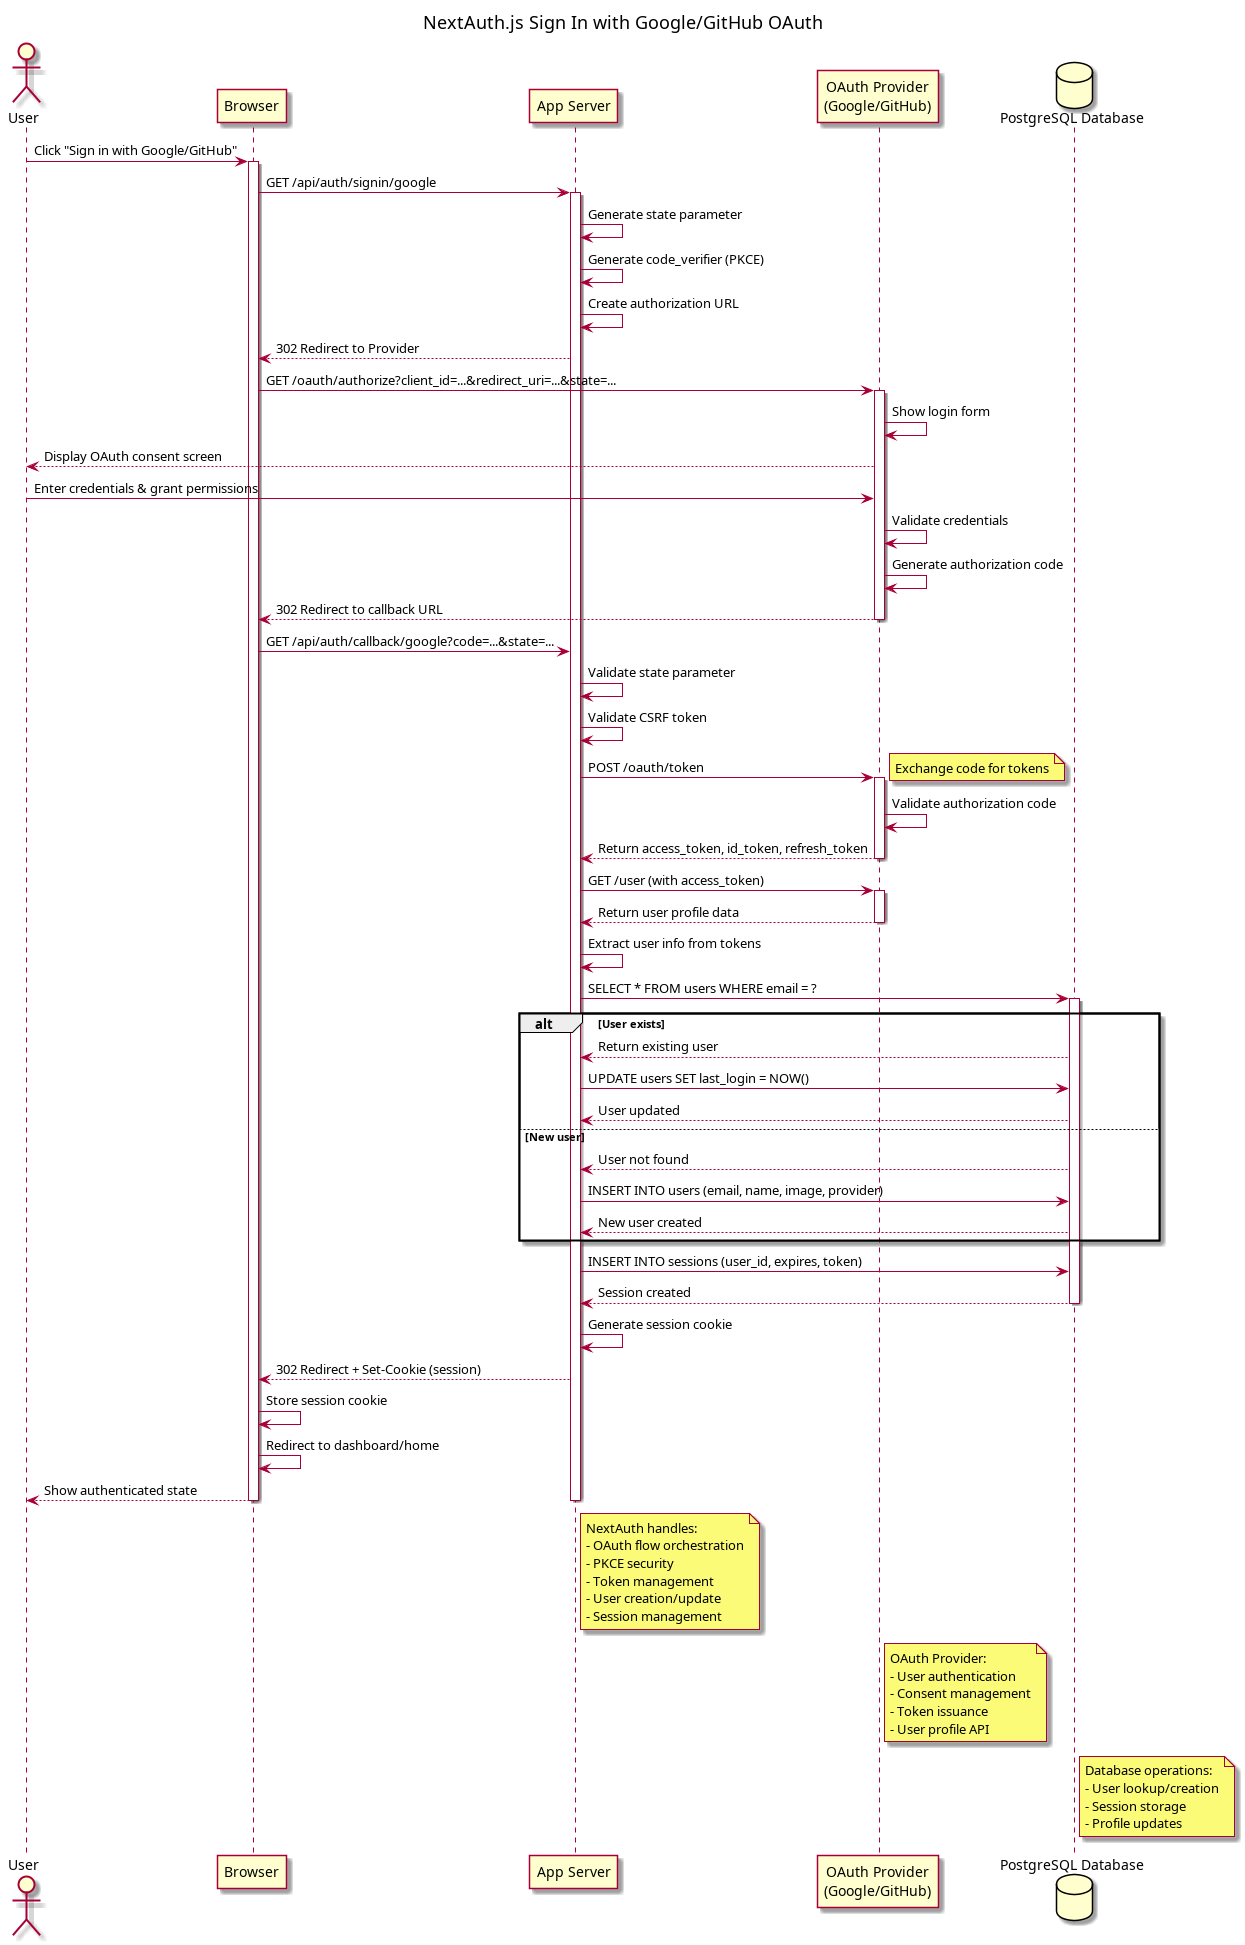
\includegraphics[width=1.0\textwidth]{conception/SprintII/sequence_diagrams/sequence_authentication_1_1_AuthenticateUsingGoogleAccount.png}
    \caption{Sequence Diagram - Google Authentication}
    \label{fig:seq_google_auth}
\end{figure}

The sequence diagram illustrates the OAuth 2.0 flow for Google authentication, showing the interaction between the user, client application, authorization server, and resource server.

\textbf{Stay Authenticated Across Devices}
\begin{figure}[H]
    \centering
    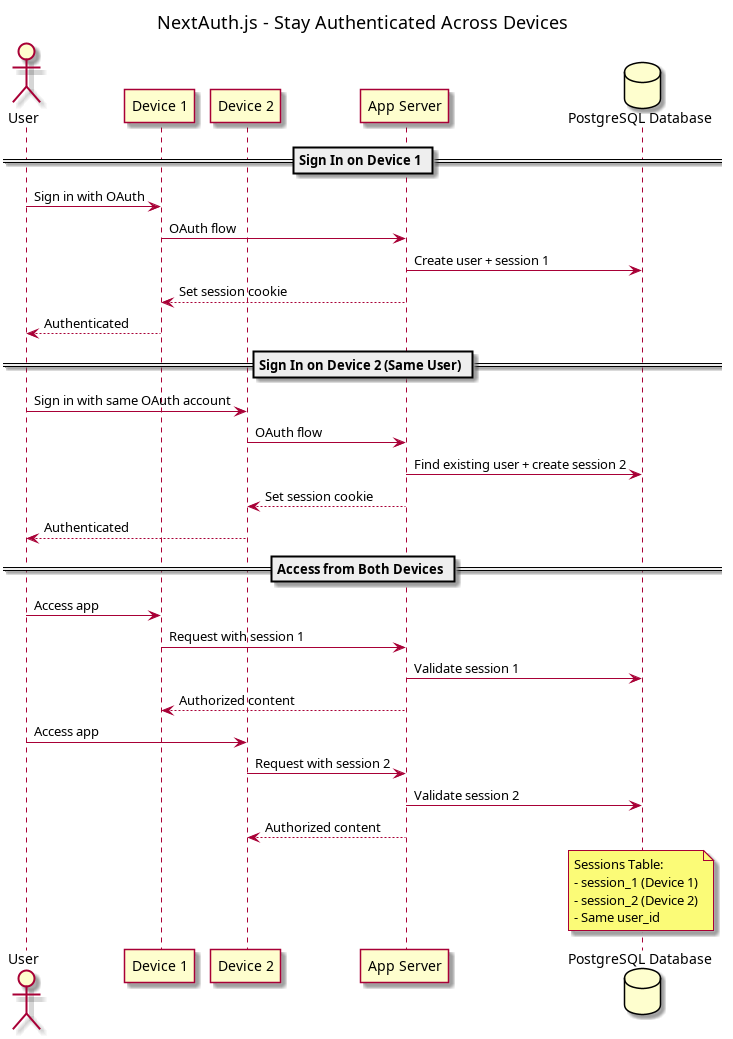
\includegraphics[width=1.0\textwidth]{conception/SprintII/sequence_diagrams/sequence_authentication_1_3_StayAuthenticatedAcrossDevices.png}
    \caption{Sequence Diagram - Cross-Device Authentication}
    \label{fig:seq_cross_device}
\end{figure}

This sequence diagram demonstrates how the application maintains user sessions across multiple devices using persistent tokens and session validation mechanisms.

\textbf{Sign Out From Account}
\begin{figure}[H]
    \centering
    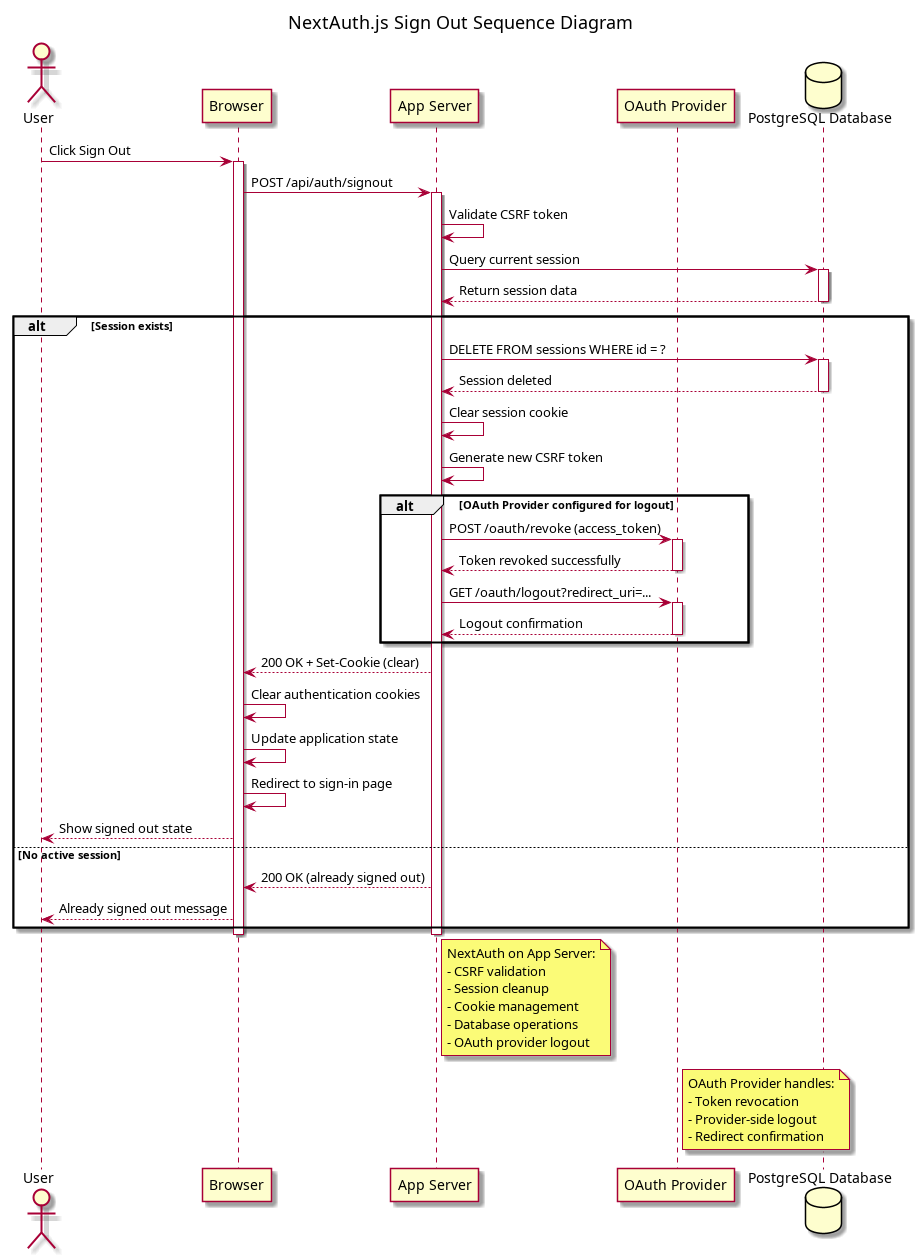
\includegraphics[width=1.0\textwidth]{conception/SprintII/sequence_diagrams/sequence_authentication_1_4_SignoutFromAccount.png}
    \caption{Sequence Diagram - Sign Out Process}
    \label{fig:seq_signout}
\end{figure}

The sign-out sequence diagram shows the secure termination of user sessions, including token invalidation and cleanup processes.

\section{Deliverables of Sprint II}

The following screenshots demonstrate the key deliverables implemented during Sprint II:

\textbf{Landing Page}
\begin{figure}[H]
    \centering
    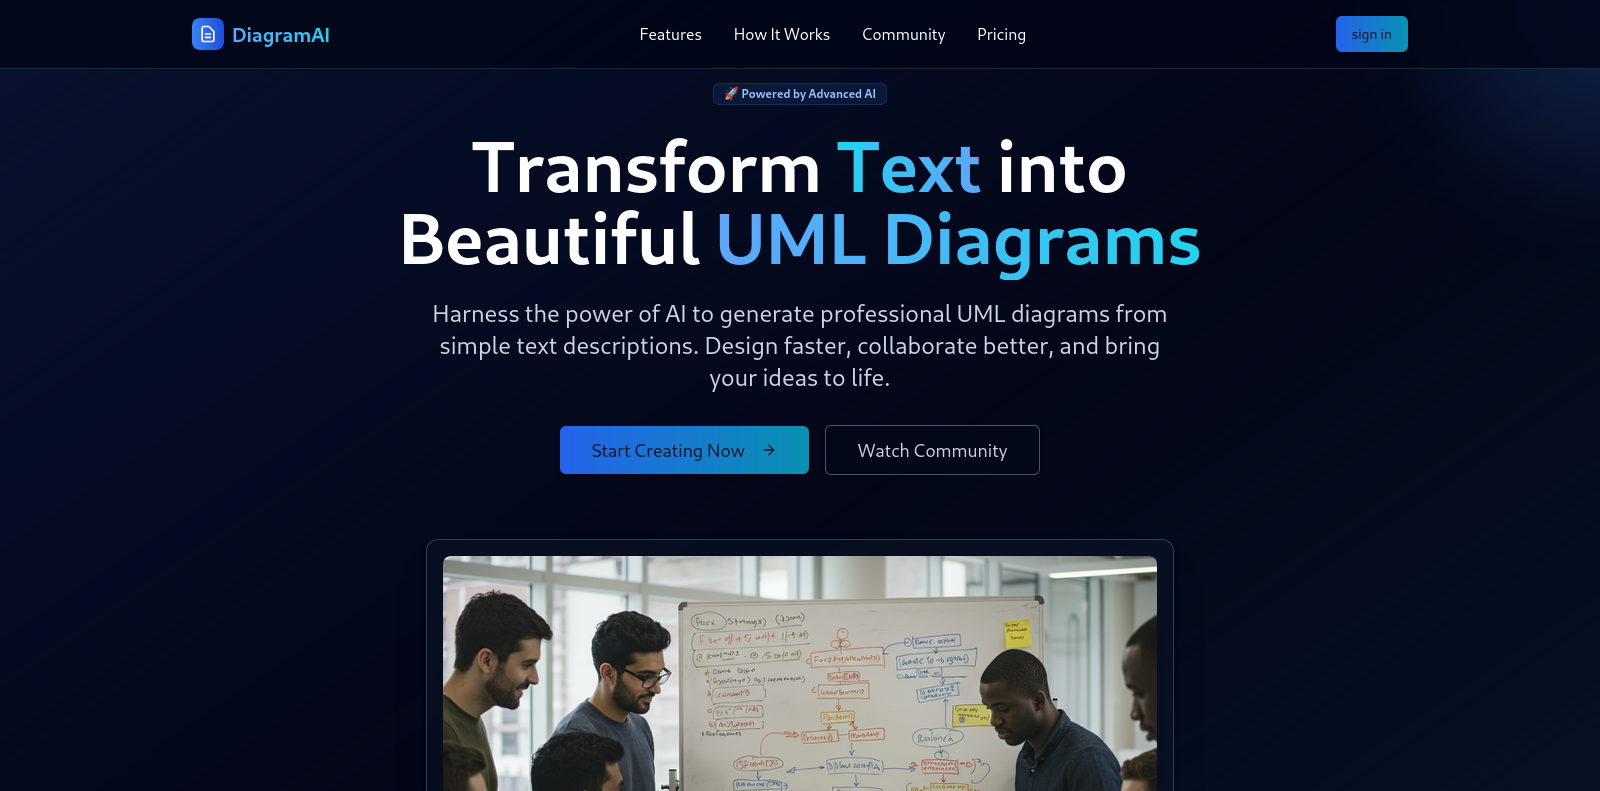
\includegraphics[width=1.0\textwidth]{screenshots/landing.png}
    \caption{Landing Page Implementation}
    \label{fig:landing_page}
\end{figure}

The landing page serves as the application's entry point, featuring a modern design with clear value proposition, feature highlights, and prominent call-to-action elements.

\textbf{Sign-In Interface}
\begin{figure}[H]
    \centering
    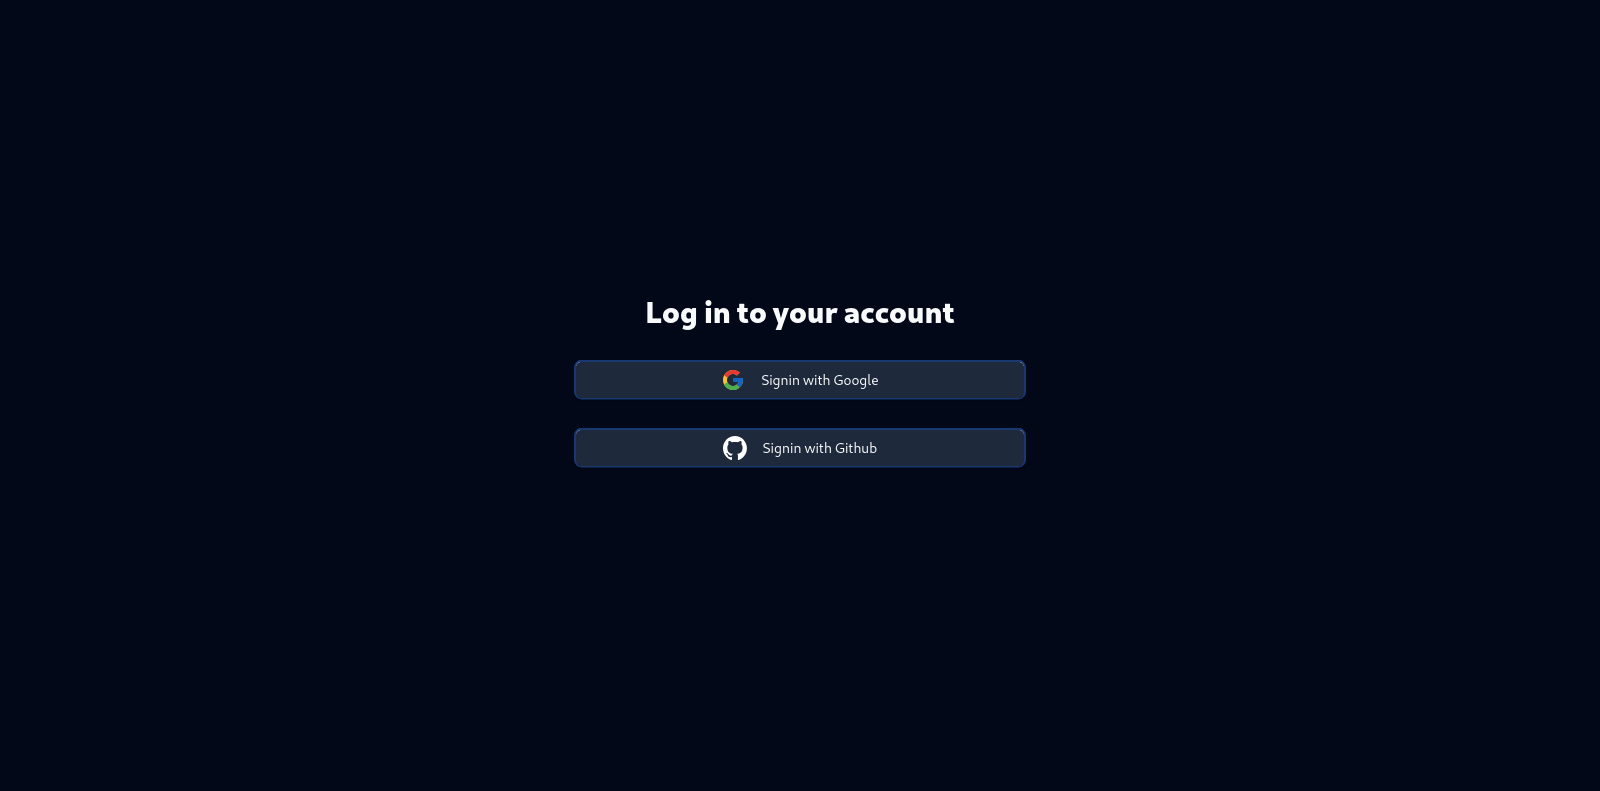
\includegraphics[width=0.8\textwidth]{screenshots/signin.png}
    \caption{Sign-In Page with OAuth Options}
    \label{fig:signin_page}
\end{figure}

The sign-in interface provides users with multiple authentication options, including Google and GitHub OAuth integration, presented in a clean and user-friendly design.

\textbf{Sign-Out Confirmation}
\begin{figure}[H]
    \centering
    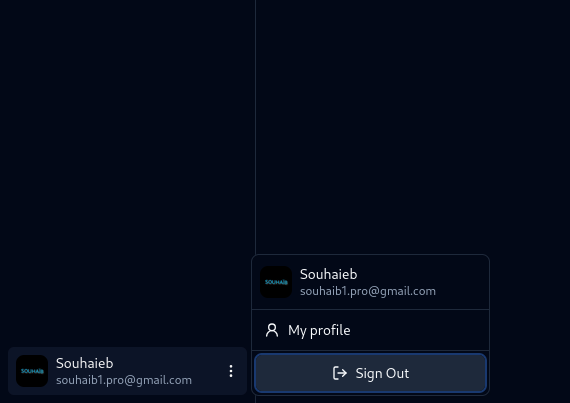
\includegraphics[width=0.8\textwidth]{screenshots/sign-out.png}
    \caption{Sign-Out Confirmation Interface}
    \label{fig:signout_page}
\end{figure}

The sign-out interface ensures users can securely terminate their sessions with appropriate confirmation mechanisms.

\section{Retrospective of Sprint II}

Sprint II successfully delivered all planned authentication features and the landing page implementation. The team effectively integrated NextAuth.js with OAuth providers, establishing a robust authentication foundation. Key achievements include seamless Google and GitHub authentication, persistent cross-device sessions, and an engaging landing page. Challenges encountered included OAuth configuration complexities and session management across different environments, which were resolved through thorough testing and documentation review. The sprint demonstrated strong collaboration between frontend and backend development, resulting in a cohesive user experience.

\section{Conclusion}

Sprint II established the essential authentication infrastructure and user entry point for the application. The successful implementation of OAuth-based authentication using NextAuth.js, combined with Prisma's database management capabilities, provides a secure and scalable foundation for user management. The responsive landing page effectively communicates the application's value proposition while guiding users toward engagement. These achievements position the project well for subsequent sprints, with a solid authentication system that supports the application's security requirements and user experience goals.